
\documentclass{article}

\usepackage{hyperref}
\usepackage{graphicx}
\usepackage{listings}

\title{Recipe Manager (0.1.1) Manual}
\author{}
\date{}

\begin{document}

\maketitle{}

\section{Introduction\label{intro}}

Recipe Manager is a program written in Java to help you manage your
recipes. Recipes are stored within files that end in ``.cb''. These
files are read and written by the Recipe Manager. To read more about
Cookbook files and recipes, see section \ref{cbr} (Cookbook Files and
Recipes).
This guide is 1/4 school project requirement, 1/4 me having fun
writing a label for a program I am proud of, 1/4 me getting practice
with \LaTeX{}, and 1/4 information about
how to use the Recipe Manager program.

\subsection{Downloading, ``Installing'', and Launching\label{downld}}

Recipe Manager .jar's are available for download at
\href{https://github.com/AshtonCross/recipeManagerJ}{the recipe
  manager github page} under the ``releases'' tab.

\begin{center}
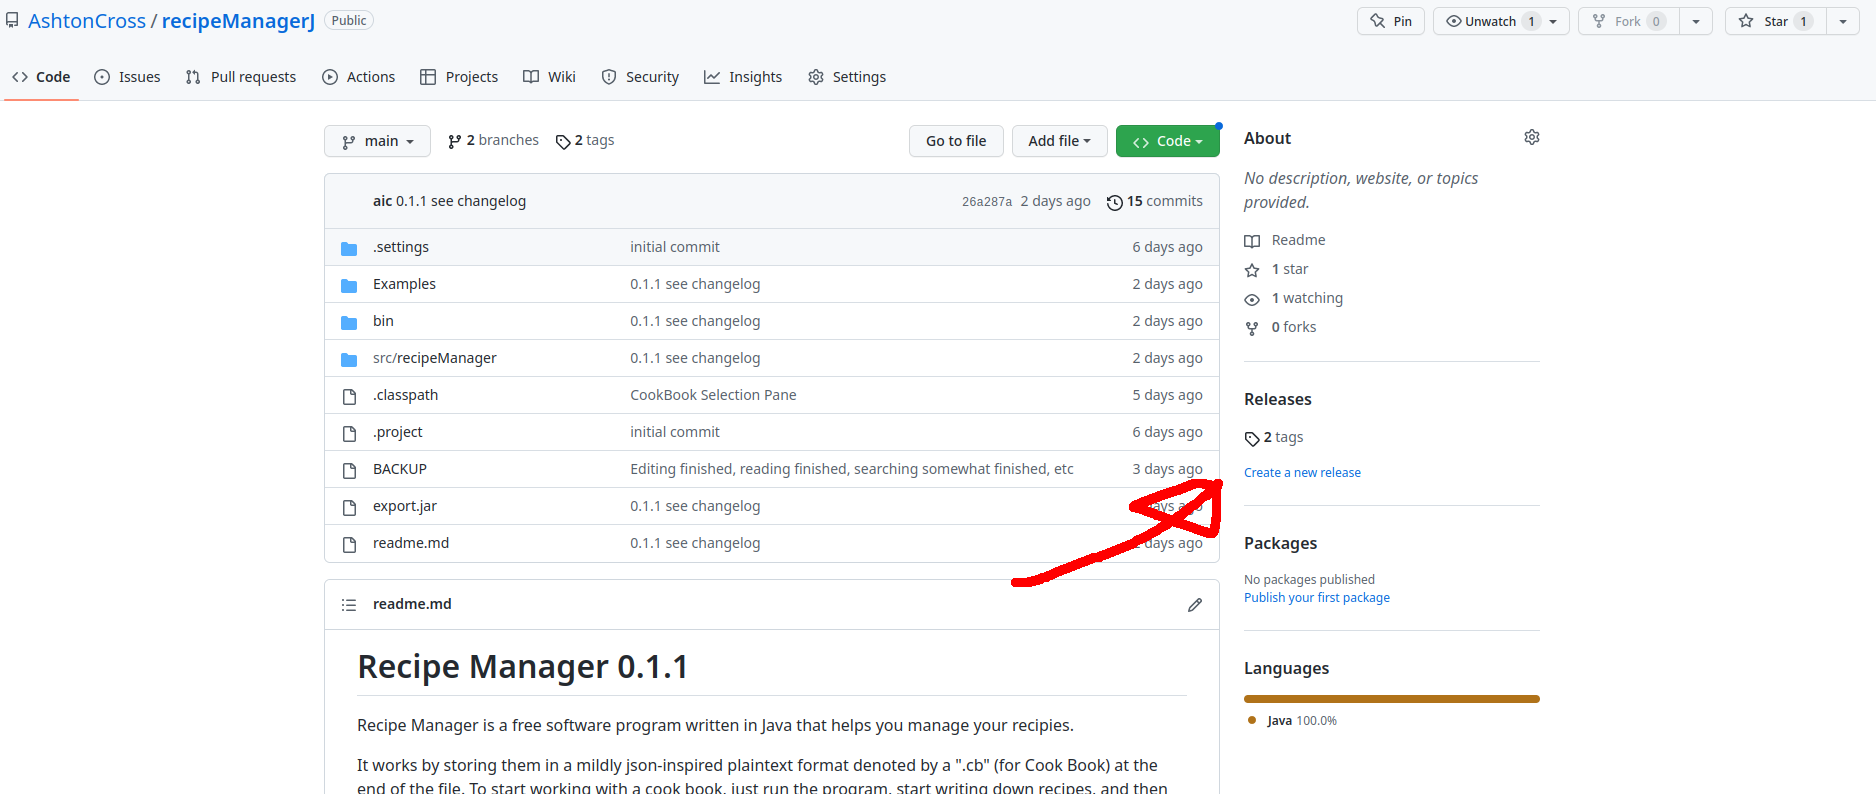
\includegraphics[width=5in]{img/releases.png}
\end{center}

After downloading the latest release, unzip the archive and move it to
a resonable location, such as in your Documents folder. Before running
the program, make sure that you have the correct version of Java
installed. Recipe Manager requires any version above Java 17. After
you have the proper Java Runtime Environment installed, you may now
run the program. 

To run the program, you now need to open a terminal and run the
following command:

\lstset{}
\begin{lstlisting}
  java -jar Recipe-Manager.jar
\end{lstlisting}

Certain systems may also allow you to double click the .jar file in a
file browser. If this is not the case with your operating system, then
I reccommend creating a run script. On Unix systems such as GNU/Linux,
this script should look something like this:

\lstset{language=bash, numbers=left, caption=run.sh}
\begin{lstlisting}
  #!/usr/bin/sh
  
  java -jar /absolute/path/to/Recipe-Manager.jar
\end{lstlisting}

After creating, give the file run permissions with the command ``chmod
+x run.sh'', and then run by entering ./run.sh into the terminal. (sh
run.sh works fine as well, and does not require executable
permissions). This script should also function on MacOSX or BSD, as
well as most other Unix operating systems with Java installed.

For Windows, you can use this exact same execution script (minus the
shebang at the first line) stored within a .bat file, so long as you
have your Java Runtime Environment in your PATH environment
variable.

\subsection{Creating Your First Recipe}

When you first launch Recipe Manager, the screen should look something
like this.

\begin{center}
  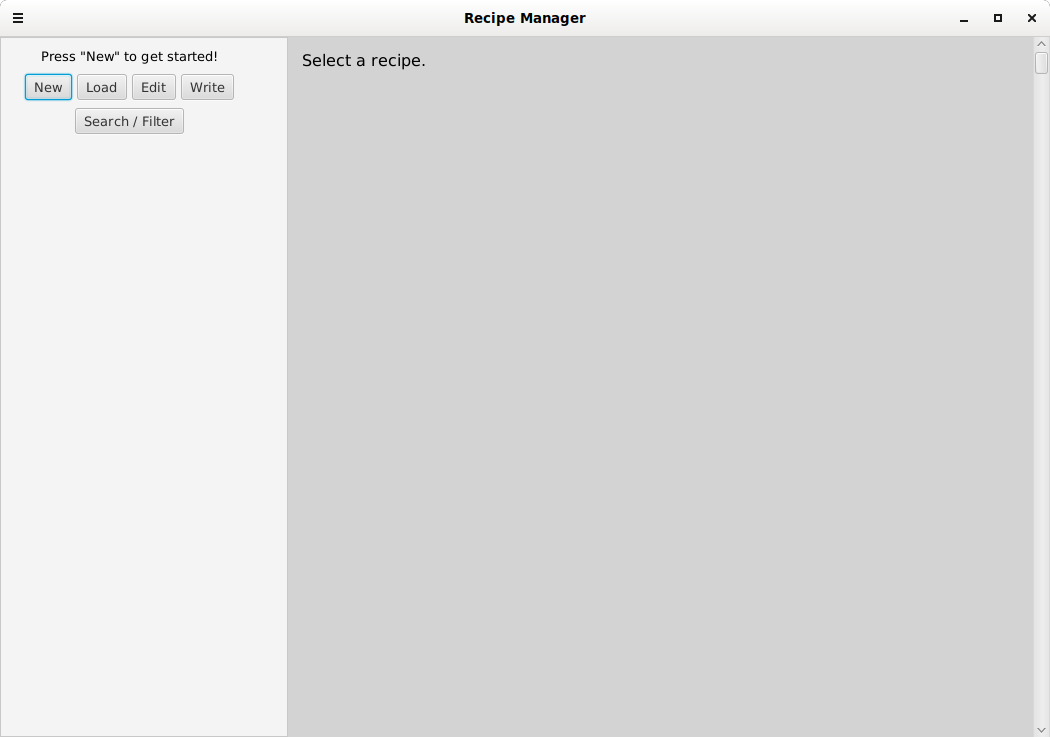
\includegraphics[width=250px]{img/emptywindow.png}
\end{center}

To create an empty recipe, click the ``New'' button. A new recipe will
appear on the Cookbook Select panel on the left. Click onto the
recipe to load it into the Information panel.

\begin{center}
  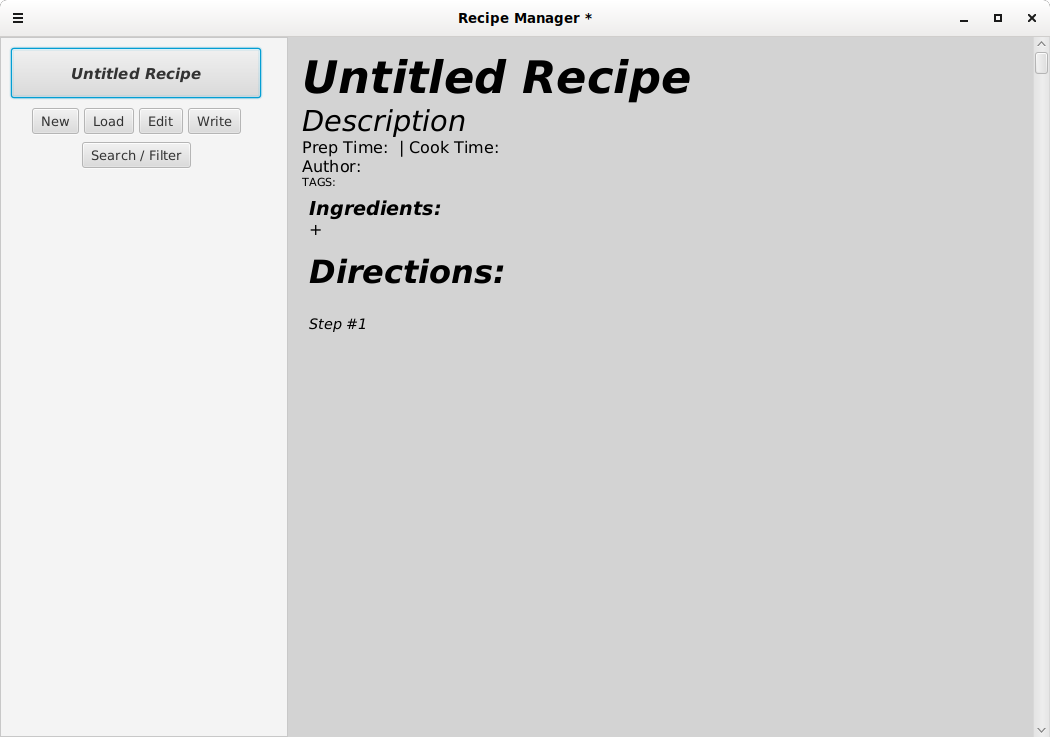
\includegraphics[width=250px]{img/newrec.png}
\end{center}

You should notice that the currently selected recipe will change its
name to bold and italic. With this recipe selected, you can now hit
the button labeled ``Edit'' to bring open the Recipe Editor.

\begin{center}
  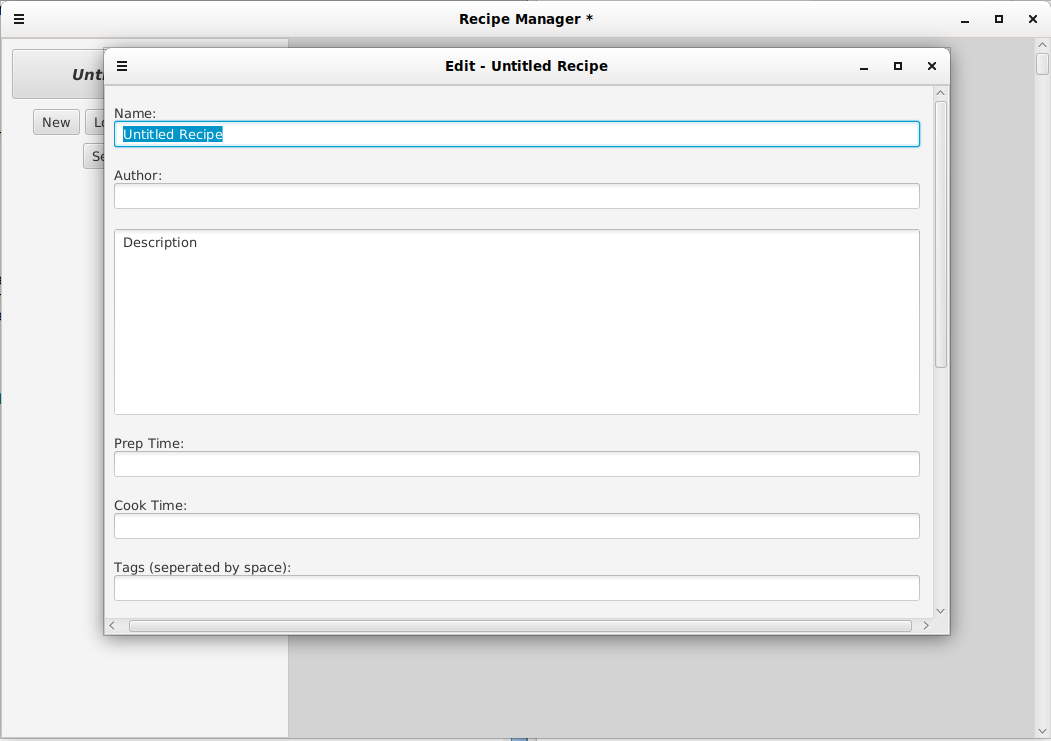
\includegraphics[width=250px]{img/editor.png}
\end{center}

This panel is where you edit a recipe. Go ahead and modify the name,
author, and description. Tags allow you to organize your recipies, for
more information, see section \ref{tags}. Incredients and directions
can be added and removed using the ``+'' and ``-'' buttons
respectivly, and then once you are done, you can click on the ``Save
Without Writing'' button. As the button implies, this will save the
recipe so that the edits are viewable from within the information
panel. You may now click on the ``Write'' button, and if you have not
written to a file yet, then it will prompt you for a location and name
for the file to be stored in.

Congratulations! You have now created a brand new recipe!

\subsection{Loading Recipes}

To load a pre-existing recipe, click the ``Load'' button on the
Control Panel. The program will prompt you for a location of a *.cb
file. After navigating to a file and selecting it, the file will then
be loaded.

\subsection{Deleting Recipes}

To delete a recipe, select the recipe that you want to delete, and
then enter the Editor by hitting the ``Edit'' button on the Control
Panel. After entering the Editor, scroll down to the bottom of the
Editor, and click the ``Delete'' button. The program will ask you if
you are sure, and after confirmation, the recipe will be removed from
the list. This recipe will not be written the next time that the
``Write'' button is envoked. 

\section{Cookbook Files and Recipes\label{cbr}}

Cookbook files, denoted by the file postfix ``.cb''. These files are
plaintext, and are editable via any text-editor. 

\begin{center}
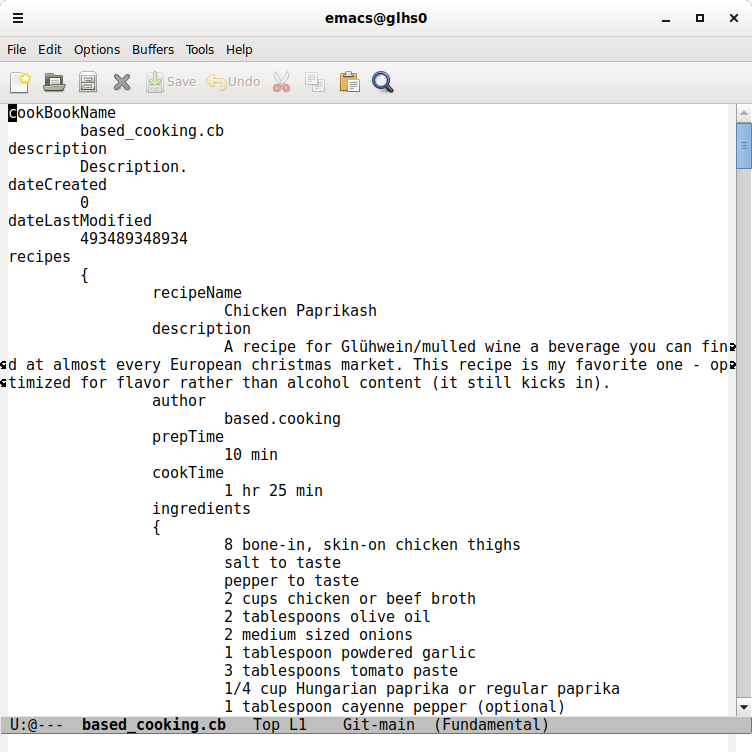
\includegraphics[width=250px]{img/emac.png}
\end{center}

It is best not to tamper with the data within the plaintext file, as
the Recipe Manager interpretor is very sensitive to indentation.

\subsection{Recipes}

Recipes contain the following information:

\begin{itemize}
\item{Name of the recipe.}
\item{Author name.}
\item{Description of recipe.}
\item{Prep time.}
\item{Cook time.}
\item{Tags\textsuperscript{ \ref{tags} }. }
\item{Ingredients.}
\item{Directions.}
\end{itemize}

The first few elements of the recipe do not have any special
formatting and are displayed and stored as-is. The ingredients and
directions are expandable, and you may add as many additional
directions and ingredients as needed. 

\subsection{Tags\label{tags}}

Tags are used for sorting recipes. Recipes are given tags, and when
searching by tags, only recipes with that tag will show up on the
Control Panel. To search, simply click the intuitivly labeled ``Search
/ Filter'' button on the Control Panel. From there the Filter Menu
will open up.

\begin{center}
  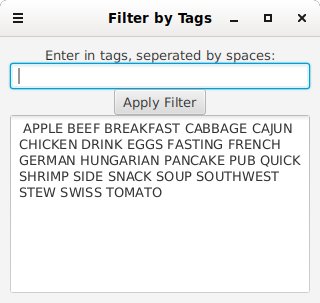
\includegraphics[width=150px]{img/filter.png}
\end{center}

The text area showcases every avalible tag currently used by recipes
currently loaded into the frame.

\section{Compiling Source}

For building, I recommend compiling the project through Eclipse. Start
by importing the project into Eclipse, then right click on the project
in the Package Explorer, and click ``Export''. Continue on with all
the default values, then it should create a jar file called
``Export.jar'' located in the project files.

Run this file using the instructions in section \ref{downld}.

\end{document}